\chapter{Elliptic Curve Theory}

\section{A Puzzle of Squares and Pyramids}

Consider the following question:\begin{quote}
``What is the number of balls that may be piled as a square pyramid and also re-arranged into a square array?''
\end{quote}
To address this, let \( x \) be the height of the pyramid. The number of balls in a pyramid of height \( x \) is given by:
\[
1^2 + 2^2 + 3^2 + \ldots + x^2 = \frac{x(x+1)(2x+1)}{6}
\]
We seek a configuration where this sum also forms a perfect square, i.e.,
\[
y^2 = \frac{x(x+1)(2x+1)}{6}
\]
This equation forms the basis of our puzzle, intertwining the concepts of geometric and numeric squares.
\vspace{24pt}
\begin{center}
	\begin{tikzpicture}[scale=1]
		\begin{axis}[
			axis lines=middle,
			xlabel=$x$,
			ylabel=$y$,
			ymin=-1.25, ymax=1.25,
			xmin=-1.25, xmax=1.25,
			domain=-1.25:1.25,
			samples=1000,
			grid=both,
			grid style={line width=.1pt, draw=gray!10},
			major grid style={line width=.1pt,draw=gray!50},
			]
			\addplot [red, smooth, thick, name path=A] {sqrt(x*(x+1)*(2*x+1)/6)};
			\addplot [red, smooth, thick, name path=B] {-sqrt(x*(x+1)*(2*x+1)/6)};
			%		\addplot [fill=blue!10] fill between[of=A and B];
		\end{axis}
	\end{tikzpicture}
\end{center}

\newpage
\subsection{Diophantus' Approach}

We consider a set of known points to produce new points. The trivial solutions \( (0,0) \) and \( (1,1) \) fit the equation of the line \( y = x \). 
\begin{center}
	\begin{tikzpicture}[scale=1]
		\begin{axis}[
			axis lines=middle,
			xlabel=$x$,
			ylabel=$y$,
			ymin=-1.25, ymax=1.25,
			xmin=-1.25, xmax=1.25,
			domain=-1.25:1.25,
			samples=1000,
			grid=both,
			grid style={line width=.1pt, draw=gray!10},
			major grid style={line width=.1pt,draw=gray!50},
			]
			\addplot [red, smooth, thick, name path=A] {sqrt(x*(x+1)*(2*x+1)/6)};
			\addplot [red, smooth, thick, name path=B] {-sqrt(x*(x+1)*(2*x+1)/6)};
			\addplot [blue, smooth, thick, name path=A] {x};
			
			\addplot[mark=*, mark options={fill=red, scale=1.5}] coordinates {(1,1)};
			\node[above left] at (axis cs:1,1) {(1,1)};
			\addplot[mark=*, mark options={fill=red, scale=1.5}] coordinates {(0,0)};
			\node[above left] at (axis cs:0,0) {(0,0)};
			
			\addplot[mark=x, mark options={fill=blue, draw=blue, scale=3, line width=2pt}] coordinates {(1/2,1/2)};
			\node[below right] at (axis cs:1/2,1/2) {($\frac{1}{2}$,$\frac{1}{2}$)};
			%		\addplot [fill=blue!10] fill between[of=A and B];
		\end{axis}
	\end{tikzpicture}
\end{center}

Intersecting this line with the curve described by our pyramid problem, we rearrange terms:
\begin{align*}
\frac{x(x+1)(2x+1)}{6}&=x^2,\\
(x^2+x)(2x+1)&=6x^2,\\
2x^3+x^2+2x^2+x&=6x^2,\\
x(2x^2-3x+1)&=0,\\
x(x-1)(2x-1)&=0.
\end{align*}

We find that \( x = \frac{1}{2} \) is a solution, implying \( y = \frac{1}{2} \). The symmetry of the curve also yields \( \left(\frac{1}{2}, -\frac{1}{2}\right) \) as another solution.

\subsection{Extending Diophantus' Method}

Consider the line through \( \left(\frac{1}{2}, -\frac{1}{2}\right) \) and \( (1,1) \), which implies \( y = 3x - 2 \). 
\begin{center}
	\begin{tikzpicture}[scale=1]
		\begin{axis}[
			axis lines=middle,
			xlabel=$x$,
			ylabel=$y$,
			ymin=-1.25, ymax=1.25,
			xmin=-1.25, xmax=1.25,
			domain=-1.25:1.25,
			samples=1000,
			grid=both,
			grid style={line width=.1pt, draw=gray!10},
			major grid style={line width=.2pt,draw=gray!50},
			]
			\addplot [red, smooth, thick, name path=A] {sqrt(x*(x+1)*(2*x+1)/6)};
			\addplot [red, smooth, thick, name path=B] {-sqrt(x*(x+1)*(2*x+1)/6)};
			\addplot [blue, smooth, thick, name path=A] {3*x-2};
			
			\addplot[mark=*, mark options={fill=green, scale=1.5}] coordinates {(1,1)};
			\node[above left] at (axis cs:1,1) {(1,1)};
			\addplot[mark=*, mark options={fill=green, scale=1.5}] coordinates {(1/2,-1/2)};
			\node[below right] at (axis cs:1/2,-1/2) {($\frac{1}{2}$,$-\frac{1}{2}$)};
			
			%		\addplot [fill=blue!10] fill between[of=A and B];
		\end{axis}
	\end{tikzpicture}
\end{center}

Intersecting this with our curve, we derive:

\begin{equation}
	x^3 - \frac{51}{2}x^2 + \ldots = 0
\end{equation}

This leads to the solutions \( x = 24 \) and \( y = 70 \), demonstrating the power of algebraic manipulation and geometric insight.

\newpage
\section{Why is it called an Elliptic Curve?}
%\begin{tikzpicture}
%	% Axes
%	\draw[->] (-3,0) -- (3,0) node[right] {$w$};
%	\draw[->] (0,-3) -- (0,3) node[above] {$y$};
%	
%	% Sine function
%	\draw[domain=-3:3, smooth, variable=\x, blue] plot ({\x}, {sin(deg(\x))});
%	\node[blue] at (2,1.5) {$y = \sin w$};
%	
%	% Inverse Sine function (integral representation)
%	\fill[red, opacity=0.3] (0,0) -- plot[domain=0:0.5] ({\x}, {sin(deg(\x))}) -- (0.5,0) -- cycle;
%	\node[red] at (1,-1) {$w(y) = \sin^{-1} y$};
%	
%	% Abel's function
%	\draw[domain=-0.99:0.99, smooth, variable=\x, green] plot ({\x*3}, {3*sqrt(1-\x*\x)});
%	\node[green] at (-2,2.5) {$F(w)$};
%\end{tikzpicture}

The term ``elliptic curve'' has its roots in the quest to measure the circumference of an ellipse. Consider the trigonometric function \( y = \sin w \). The inverse function, \( w(y) = \sin^{-1} y \), is expressed as an integral:
\[
w(y) = \sin^{-1} y = \int_{0}^{y} \frac{1}{\sqrt{1 - t^2}} \, dt
\]
This integral is foundational in understanding the link between elliptic curves and elliptic integrals.

\subsection{Abel's Insight}
Niels Henrik Abel, a prominent mathematician, extended this concept. Starting with \( y = \sin w \), Abel explored the inverse functions of elliptic integrals, uncovering their double periodicity. He defined the function:
\[
F(w) = \int_{0}^{w} \frac{dz}{\sqrt{(1 - z^2)(1 - k^2 z^2)}}
\]
Abel's work laid the groundwork for understanding the complex nature of elliptic curves.

\subsection{The Geometry of an Ellipse}

An ellipse is defined by the equation \( x^2/a^2 + y^2/b^2 = 1 \). This simple equation belies the complexity of calculating its arc length.

\subsection{The Arc Length of an Ellipse}

Defining \( k^2 = 1 - \frac{b^2}{a^2} \) and changing variables \( x \rightarrow ax \), we express the arc length of an ellipse as:
\[
a \int_{-1}^{1} \sqrt{\frac{1 - k^2 x^2}{1 - x^2}} \, dx = a \int_{-1}^{1} \frac{1 - k^2 x^2}{\sqrt{(1 - x^2)(1 - k^2 x^2)}} \, dx
\]
This leads to the following representation of the arc length:
\[
\textbf{Arc Length} = a \int_{-1}^{1} \frac{1 - k^2 x^2}{y} \, dx\quad\text{with}\quad y^2=(1-x^2)(1-k^2x).
\]

\subsection{Connecting to an Elliptic Curve}

The ellipse's arc length calculation brings us to a critical realization. An elliptic integral is generally expressed as:
\[
\int R(x,y) \, dx
\]
This integral, deeply connected to the geometry of ellipses, underpins the theory of elliptic curves.

\newpage
\section*{Double Periodicity in Elliptic Curves}

Elliptic curves are intimately connected with the study of complex tori, which can be represented through the use of doubly periodic functions. A fundamental example of such a function is the Weierstrass $\wp$ function, defined by a lattice $\Lambda$ in the complex plane. 

\subsection*{The Weierstrass $\wp$ Function}

Given a lattice $\Lambda \subset \mathbb{C}$, the Weierstrass $\wp$ function is defined as:
\begin{equation}
	\wp(z; \Lambda) = \frac{1}{z^2} + \sum_{\omega \in \Lambda \setminus \{0\}} \left( \frac{1}{(z - \omega)^2} - \frac{1}{\omega^2} \right).
\end{equation}

This function is even, $\wp(-z) = \wp(z)$, and exhibits double periodicity with respect to the lattice $\Lambda$, meaning:
\begin{equation}
	\wp(z + \omega) = \wp(z) \quad \text{for all} \, \omega \in \Lambda.
\end{equation}

\subsection*{Elliptic Curves and the $\wp$ Function}

An elliptic curve can be associated with the Weierstrass $\wp$ function. Specifically, an elliptic curve over $\mathbb{C}$ can be described in the Weierstrass form:
\begin{equation}
	y^2 = 4x^3 - g_2x - g_3,
\end{equation}
where $g_2$ and $g_3$ are constants derived from the lattice $\Lambda$. The coordinates $(x, y)$ on the elliptic curve correspond to the values of the Weierstrass $\wp$ function and its derivative:
\begin{equation}
	x = \wp(z; \Lambda), \quad y = \wp'(z; \Lambda).
\end{equation}


\section*{Double Periodicity}

\subsection*{Two linearly independent periods.}
\[
\phi(z + w_1) = \phi(z + w_2) = \phi(z) \text{ for all complex number } z.
\]

\subsection*{It satisfies}
\[
[\phi'(z)]^2 = 4\phi(z)^3 - 60 G_4 \phi(z) - 140 G_6
\]

\begin{itemize}
	\item So for $x=\phi(z)$ and $y=\phi'(z)$
	\item $y^2=4x^3-60G_3x-140G_6$
\end{itemize}


\newpage
\section*{Elliptic Functions and Elliptic Curves}

The \(\wp\)-function and its derivative satisfy an algebraic relation
\[
\wp'(z)^2 = \wp(z)^3 + A \wp(z) + B
\]

The double periodicity means that it is a function on the quotient space \(\mathbb{C}/\Lambda\), where \(\Lambda\) is the lattice
\[
\Lambda = \{ n_1\omega_1 + n_2\omega_2 : n_1,n_2\in\mathbb{Z}\}.
\]
\vspace{8pt}
\begin{center}
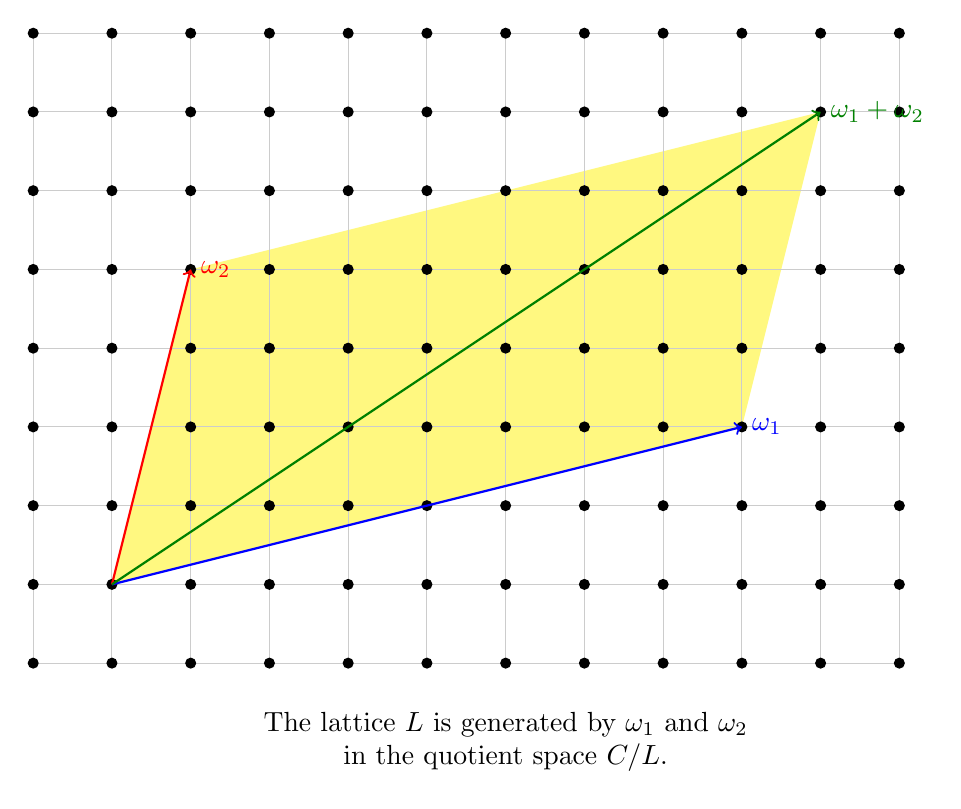
\begin{tikzpicture}[scale=1]
	\fill[yellow!50] (-4,-3) -- (4,-1) -- (5,3) -- (-3,1) -- cycle;
	\draw[thin,gray!40] (-5,-4) grid (6,4);
	% Draw axes
%	\draw[->] (-2,0) -- (4,0) node[right] {$\Re$}; % Real axis
%	\draw[->] (0,-2) -- (0,4) node[above] {$\Im$}; % Imaginary axis
	
	% Define lattice points
	\foreach \x in {-5,...,6} \foreach \y in {-4,...,4} {
		\fill (\x,\y) circle (2pt); % Lattice points
	}
	
	\draw[blue,thick,->] (-4,-3) -- (4,-1) node[right] {$\omega_1$};
	\draw[red,thick,->] (-4,-3) -- (-3,1) node[right] {$\omega_2$};
	\draw[green!50!black,thick,->] (-4,-3) -- (5,3) node[right] {$\omega_1+\omega_2$};
	 \node[align=center] at (1,-5) {The lattice $L$ is generated by $\omega_1$ and $\omega_2$\\in the quotient space $\mathbb{C}/L$.};
\end{tikzpicture}
\end{center}
\section*{Elliptic Functions and Elliptic Curves}

Elliptic functions and elliptic curves are fundamental objects in complex analysis and algebraic geometry, respectively. They are interconnected through the Weierstrass $\wp$ function and its properties.

\subsection*{Weierstrass Elliptic Functions}

The Weierstrass elliptic functions are defined with respect to a lattice $\Lambda \subset \mathbb{C}$. The Weierstrass $\wp$ function, a key example of an elliptic function, is defined as:
\begin{equation}
	\wp(z; \Lambda) = \frac{1}{z^2} + \sum_{\omega \in \Lambda \setminus \{0\}} \left( \frac{1}{(z - \omega)^2} - \frac{1}{\omega^2} \right).
\end{equation}
This function is doubly periodic and meromorphic with poles of order two at lattice points.

\subsection*{Elliptic Curves and the Weierstrass $\wp$ Function}

An elliptic curve can be described as a set of points satisfying a cubic equation in two variables. Over the complex numbers, this curve can be associated with the Weierstrass $\wp$ function.

An elliptic curve in Weierstrass form is given by:
\begin{equation}
	y^2 = 4x^3 - g_2x - g_3,
\end{equation}
where $g_2$ and $g_3$ are constants determined by the lattice $\Lambda$. The function $\wp$ and its derivative relate to the curve as follows:
\begin{align}
	x &= \wp(z; \Lambda), \\
	y &= \wp'(z; \Lambda).
\end{align}
This establishes a correspondence between points on the complex torus $\mathbb{C}/\Lambda$ and points on the elliptic curve.

\subsection*{Properties of Elliptic Curves}

Elliptic curves have several important properties:

\begin{itemize}
	\item They form a group under a geometrically defined addition operation.
	\item The addition operation on the curve corresponds to the addition of points in the complex plane modulo the lattice $\Lambda$.
	\item Elliptic curves over finite fields have applications in number theory and cryptography.
\end{itemize}


\newpage
\section*{The Complex Points on an Elliptic Curve}

The \(\phi\)-function gives a complex analytic isomorphism
\[
\frac{\mathbb{C}}{L} = \big(\phi(z),\phi'(z)\big) \rightarrow E(\mathbb{C})
\]
with the notation that \( \mathbb{C} \) is the complex numbers, \( L \) is a lattice, and \( E(\mathbb{C}) \) is the set of complex points on an elliptic curve.

%\begin{figure}[h!]
%	\centering
%	\includegraphics[width=0.5\textwidth]{parallelogram_to_torus.png}
%	\caption{Parallelogram with opposite sides identified = a torus.}
%\end{figure}

Thus the points of \( E \) with coordinates in the complex numbers \( \mathbb{C} \) form a \textit{torus}, that is, the surface of a donut.

%\begin{figure}[h!]
%	\centering
%	\includegraphics[width=0.5\textwidth]{torus.png}
%	\caption{The complex points \( E(\mathbb{C}) \) forming a torus.}
%\end{figure}

\section*{X\(^2\) + Y\(^2\) = C}

\begin{itemize}
	\item Let \( x = a + b\sqrt{-1} \), \( y = c + d\sqrt{-1} \).
	\item The solution over complex numbers is a surface, in fact topologically sphere.
	\item If unbelievable, check out level curves.
	\item Furthermore, it has group structure.
	\[ (a + b\sqrt{-1})(c + d\sqrt{-1}) \text{ becomes } ac-bd + (ad+bc)\sqrt{-1} \]
\end{itemize}

\section*{Why is it called Torus?}
\begin{itemize}
	\item Complex Tori \[
	y^2=x(x^2-1)
	\]
	\item If we introduce \textit{points at infinity} and the \textit{complex numbers}, we can argue that the graph is a torus.
\end{itemize}

\section*{Why Elliptic Curve?}

\begin{itemize}
	\item Discrete Logarithm Problem
	\item Given a finite group \( G \) with two of its elements \( a \) and \( b \).
	\item Find an integer \( x \) such that, \( a^x = b \) if it exists.
	\item Example: Non-zero elements of some finite field.
\end{itemize}

\section*{Better groups?}

For a finite field \( F \),
\[
GL_2(F) = \left\{ \begin{pmatrix}
	a & b \\
	c & d
\end{pmatrix} \mid ad - bc \neq 0, \, a,b,c,d \in F \right\}
\]

\begin{itemize}
	\item The Times(London) Jan. 1999 An Irish schoolgirl Sarah Flannery used matrices as an alternative to RSA. Her algorithm is far faster than the RSA and equally secure.
	\item The Art of Computer Programming by Donald Knuth
\end{itemize}

How about this group?

\begin{itemize}
	\item \( F = \mathbb{Z} / 17\mathbb{Z} = \mathbb{Z} \text{ (mod 17)} \)
	\item \( 6^2 = 36 \equiv 2 \text{ mod 17} \)
	\item \( 6 \text{ behaves like } \sqrt{2} \)
\end{itemize}

\( X^2 - 2Y^2 = 1 \)

\( (3 + 2 \sqrt{2})(3 - 2 \sqrt{2}) = 1 \)

\( (3 + 12)(3 - 12) = -36 \equiv 1 \text{ mod 17} \)



\begin{itemize}
	\item 
	Let \( G = \{(x, y) \mid x^2 - 2y^2 = 1 \text{ over } \mathbb{F}\} \) The operation on \( G \) is defined as:
	\[
	(x_1, y_1) \cdot (x_2, y_2) =
	\]
	\[
	\left( x_1 + \sqrt{2} y_1 \right) \left( x_2 + \sqrt{2} y_2 \right) =
	\]
	\[
	= \left( x_1 x_2 + 2y_1 y_2 \right) + \sqrt{2} \left( x_1 y_2 + x_2 y_1 \right)
	\]
	\[
	(x_1, y_1) \cdot (x_2, y_2) =
	\]
	\[
	= \left( x_1 x_2 + 2y_1 y_2 \right) x_1 y_2 + x_2 y_1
	\]
\end{itemize}

\section*{Why Elliptic Curve?}

\begin{itemize}
	\item DLP (Discrete Logarithm Problem) on finite field can be solved faster than we thought!
	\item by ``index calculus''
	\item To protect against this attack...
	\item Elliptic curves!
\end{itemize}



\newpage
\begin{tikzpicture}[scale=.5, >=Stealth]
	% Grid
	\draw[thin,gray!40] (-10,-10) grid (10,10);
	% Axes
	\draw[thick,<->] (-10,0)--(10,0) node[right]{$x$};
	\draw[thick,<->] (0,-10)--(0,10) node[above]{$y$};
	% Points
	% Here you would place the points you want to plot, for example:
	 \node[draw,circle,inner sep=2pt,fill] at (1,2) {};
	 \node[draw,circle,inner sep=2pt,fill] at (2,3) {};
	 \node[draw,circle,inner sep=2pt,fill] at (3,6) {};
	
	% If you have integer solutions for x and y, you would add them here.
	% For instance, if you had a solution (x,y) = (2,4), you would add:
	 \node[draw,circle,inner sep=2pt,fill] at (2,4) {};
	
	% Labels
	% Similarly, label them like so (for the point (2,4)):
	 \node at (2,4) [below left] {$(2,4)$};
\end{tikzpicture}


